\chapter{Introduction} \label{sec:intro}

%% P1: Multi-threading is critical and popular.
Multithreading has become pervasive and critical because of two computing
trends. First, due to the physical constraints on circuit speed, computing
platforms are having more and more cores rather than faster and faster
single-core. In order to harness the power of multi-core, developers write more
and more multithreaded programs on these platforms. Second, the emerging cloud
computing trend requires networking services (\eg, \http servers and database
servers) to process more and more requests concurrently, which also pushes
developers to write more and more multithreaded programs. These two trends will
continue and multithreading will become increaingly pervasive and critical.

%% P2: However, it is hard to get right.
Unfortunately, despite decades of effort from both academia and industry,
multithreaded programs are still notoriously difficult to get right, and these
programs are plagued with harmful concurrency bugs that can cause wrong outputs,
program crashes, security breaches, and so on. A root cause of this difficulty
is: even running on the same input, the concurrently running threads of a
program may interleave in \emph{too many} different ways, and we call these
interleavings \emph{schedules}. Considering all inputs, the number of possible
schedules is even greater. In this traditional multithreading manner, each
input may run into too many thread interleavings, and each interleaving may
process many different inputs. This messy many-to-many mapping
(Figure~\ref{fig:nondet}) makes multi-threaded programs extremely hard to
understand, test, analyze, and verify. As a result, a concurency bug hidden in
one schedule can easily bypass even advanced reliability and security techniques
in the testing lab and show up in the production runs.

%% P3: DMT: one possible approach. And its limitations.
To simplify this messy mapping, researchers have proposed an idea called
deterministic multithreading (or \dmt)~\cite{dthreads:sosp11, dpj:oopsla09,
dmp:asplos09, kendo:asplos09, coredet:asplos10} that always enforces the same
schedule on the same input. By mapping each input to only one schedule
(Figure~\ref{fig:dmt}), \dmt greatly improves reliability for multithreaded
programs on each input. However, although \dmt is useful, it is not as useful as
commonly perceived, because as we have shown in our previous
research~\cite{cui:tern:osdi10}, a typical \dmt system can map slightly
different inputs to very different schedules, artificially reducing programs'
robustness on input perturbation, and the number of possible schedules on all
inputs are still enormous, and the resultant programs are still very hard to
test, analyze, verify, and so on.
%Chapter~\ref{sec:related} will analyze these
%systems in more details.

\begin{figure*}[t]
\begin{center}
\subfloat[{\em
Traditional.}]{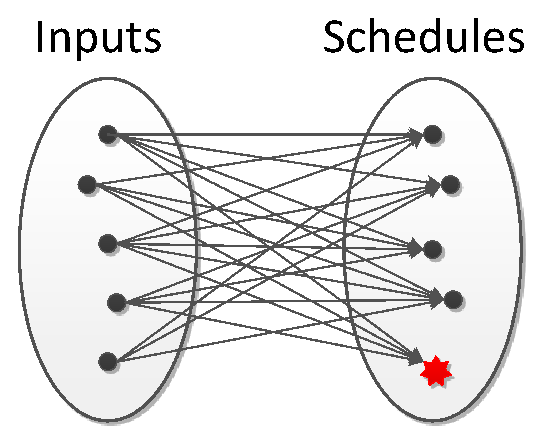
\includegraphics[width=.23\linewidth]{figures/nondet}
  \label{fig:nondet}}
\subfloat[{\em
Deterministic.}]{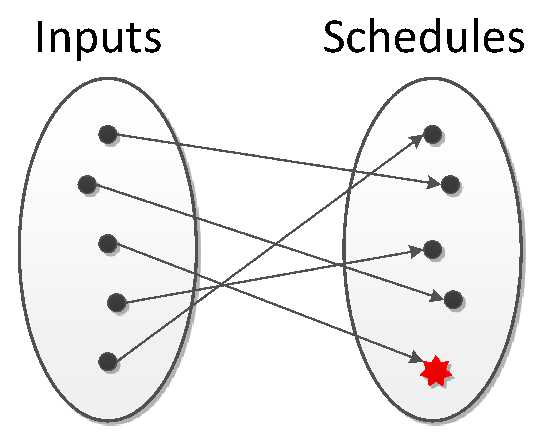
\includegraphics[width=.23\linewidth]{figures/dmt}
  \label{fig:dmt}}
\subfloat[{\em Stable
(deterministic).}]{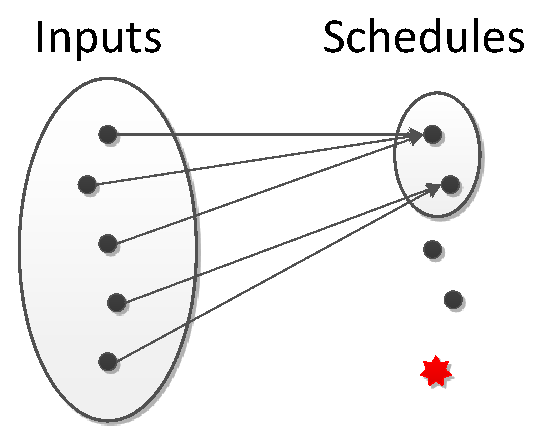
\includegraphics[width=.23\linewidth]{figures/smt}
  \label{fig:smt}}
\subfloat[{\em Stable
(nondeterministic).}]{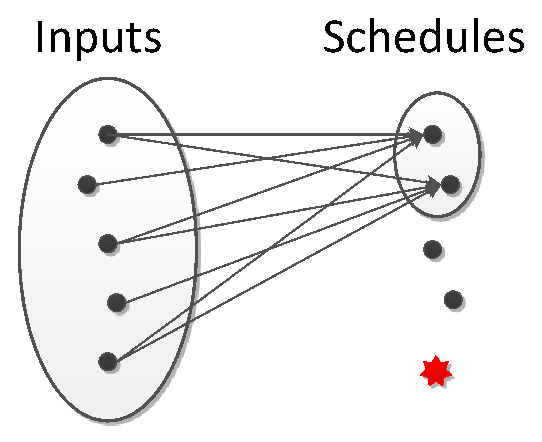
\includegraphics[width=.23\linewidth]{figures/smtn}
  \label{fig:smtn}}
\vspace{-.05in}
\caption{Different multithreading approaches. Red stars represent buggy
schedules. Traditional multithreading (\subref*{fig:nondet}) is a conceptual
many-to-many mapping where one input may execute under many schedules because of
nondeterminism, and many inputs may execute under one schedule because a
schedule fixes the order of the communication operations but allows the local
computations to operate on any input data. \dmt (\subref*{fig:dmt}) may map each
input to an arbitrary schedule, reducing programs' robustness on input
perturbations. \smt (\subref*{fig:smt} and \subref*{fig:smtn}) reduces the total
set of schedules for all inputs (represented by the shrunk ellipses), increasing
robustness and improving reliability. \smt and \dmt are orthogonal: a \smt
system can be deterministic (\subref*{fig:smt}) or nondeterministic
(\subref*{fig:smtn}).}
\vspace{-.2in}
\end{center}
\end{figure*}

%% P4: StableMT: our new approach and thesis.
In order to reduce the number of schedules for all inputs, we have studied the
relation between inputs and schedules of real-world programs, and made an
eye-opening discovery: many programs need only a small set of schedules to
efficiently process a wide range of inputs~\cite{smt:cacm}! Leveraging this
discovery, we have proposed a new idea called Stable Multi-Threading (StableMT)
that reuses each schedule on a wide range of inputs. By mapping many inputs to
the same schedule (Figure~\ref{fig:smt}), it stabilizes program behaviors
against small input perturbations and greatly reduce the number of possible
schedules for all inputs. By addressing the root cause that makes multithreading
difficult to get right, StableMT makes greatly simplifies understanding,
testing, analyzing, and verification of multithreaded programs. Note that \smt
and \dmt are complementary: a system can be both deterministic and stable.

%% P6: intro to the systems we built: with each addressing different challenges.
%%Although the vision of stable multithreading is appealing, realizing it
%%faces numerous challenges.  Three main challenges are:
To make \smt real, I have worked with Columbia and CMU researchers as a
technical leader to build three \smt (and also \dmt) systems,
\tern~\cite{cui:tern:osdi10}, \peregrine~\cite{peregrine:sosp11}, and
\parrot~\cite{parrot:sosp13}, with each addressing a distinct research
challenge. We identify and address these three challenges as follows.
%Unless specified, all our systems use a common definition for ``schedule": a
%total order of synchronization operations, such as lock acquisitions.

\para{Challenge 1: How to compute highly reusable schedules for different
inputs?} The more reusable a schedule is, the fewer schedules are needed.
However, finding highly reusable schedules is hard with existing static or
dynamic techniques, because statically computed schedules are not guaranteed to
work at runtime due to the halting problem, and dynamically computing schedules
may cause prohibitive overhead.

To address this challenge, our first \smt system, \tern~\cite{cui:tern:osdi10}
(Chapter~\ref{sec:tern}), proposes a technique called \emph{schedule
memoizatoin} that memoizes a set of past, working schedules, and then reuses
these schedules on future inputs when possible. This technique is inspired by a
real-world analogy that human and animals tend to migrate along past, familiar
routes and avoid possible hazards in unknown ones. In order to find a schedule
suitable for an input, \tern leverages a set of advanced program analysis
techniques to compute preconditions on inputs that match a schedule. Evaluation
on a diverse set of popular programs shows that \tern can reuse a small set of
schedules to process a wide range of inputs. For instance, just 100 schedules
for the \apache web server can process 90.3\% of a 4-day trace (122K requests)
from the Columbia CS website.

\para{Challenge 2: How to efficiently make executions follow schedules and do
not deviate?} This challenge has also existed in the area of deterministic
execution and replay for decades. Existing work typically enforces two types of
schedules: a total order of shared memory accesses (for short, \memsched), and a
total order of synchronization operations (for short, \syncsched). The
\memscheds are fully deterministic even with data races, but they are several
times slower than traditional multi-threading. The \syncscheds incur only modest
overhead because most code is not synchronization and thus can still run in
parallel, but these schedules may deviate if there are data races. Overall,
despite much research effort, people can only choose either full determinism or
efficiency, but not both.

To tackle this challenge, our second \smt system,
\peregrine~\cite{peregrine:sosp11} (Chapter~\ref{sec:peregrine}), stands out
with an observation: although many programs have races, the races tend to occur
only within minor portions of an execution, and the majority of the execution is
still race-free. Therefore, we can enforce a \syncscheds in the race-free
portions of an execution and resort to a \memsched only in the racy portions,
combining both the efficiency of sync-schedules and determinism of \memscheds. 
\peregrine implements hybrid-schedule with a new technique called \emph{schedule
ralaxation}. This technique first records an execution trace of all executed
instructions on a new input, and then relaxes the trace into a highly reusable
hybrid-schedule. Evaluation on a diverse set of programs shows that \peregrine
is deterministic and efficient, and can frequently reuse schedules for half of
the evaluated programs. \peregrine has been featured in sites such as
\acmtechnews, \tgdaily, and \physorg.

\para{Challenge 3: How to make \smt Simple and deployable?} In the last five
years, \smt has achieved promising advances and attracted the research
community's interest. Numerous notable \smt systems have been built, including
our \tern and  \peregrine systems. However, it remains an open challenge whether
\smt can be made simple and deployable. Existing \smt systems either run into
slow schedules that \emph{serialize} parallel computation, or are fairly hard to
deploy due to their high complexity (\eg, \tern and \peregrine require
sophisticated program analysis).

To cope with this challenge, our third \smt system, \parrot~\cite{parrot:sosp13}
(Chapter~\ref{sec:parrot}) presents a simple, deployable runtime that enforces a
well-defined round-robin schedule for synchronization operations, vastly
reducing the number of schedules. To address the serialization problem in \smt,
we come up with an insight based on the famous 80-20 rule: most threads spend
most execution time in only a few core computations, and we only need to make 
these core computations parallel. Accordingly, we create a new abstraction
called \emph{performance hints} for developers to annotate core computations.
These hints, which just try to get to faster schedules that improve parallelism
of core computations, are not real synchronization, and can be safely ignored
without affecting correctness of a program. Evaluation on a wide range of 108
popular programs (\eg, \bdb and \mplayer), roughly 10$\times$ more programs than
any prior \smt or \dmt evaluation, and about 4$\times$ more programs than all
prior evaluations combined, shows that, these hints are easy to add and make
\parrot fast (merely 12.7\% mean overhead on 24-core machines). Furthermore,
\parrot is open source for deployment.

%% P5: StableMT's applications.
%To demonstrate \smt's potential, We have quantitatively shown that
%\smt can benefit existing reliability techniques such as greatly improving
%coverage of model checking~\cite{parrot:sosp13}, making reproducing concurrency
%bugs much easier, and improving precision of static analysis~\cite{wu:pldi12}.

To demonstrate \smt's potential, we have applied \smt to improve three
reliability techniques. First, we have applied \tern to reproduce several
real-world concurrency bugs~\cite{cui:tern:osdi10}, and found that \smt's
schedules can consistently mask or reproduce these bugs, and these schedules are
stable to input perturbation. Second, we have applied \peregrine to greatly
improve the precision of program analysis~\cite{wu:pldi12} and
verification~\cite{wu:pldi12}, leading to several new harmful concurrency bugs
detected in heavily-studied programs. Third, we have quantitatively shown that
\parrot can increase the coverage by many orders of magnitudes for model
checking, an advanced technique that systematically tests schedules and try to
find bugs~\cite{parrot:sosp13, dbug:spin11, modist:nsdi09}. Each of the three
systems can benefit all these three reliability techniques with modest
engineering effort, because many techniques in our three \smt systems are
similar. For instance, \parrot can also make reproducing concurrency bugs much
more easier because it enforces a similar form of schedule to that in \tern. In
addition to our own effort on applying \smt, Some of our \smt techniques and
ideas have also been leveraged by other researchers to compute a small set of
schedules to cover all inputs for some multithreaded
programs~\cite{bergan:oopsla13}.

%Chapter~\ref{sec:related}
%introduces related work, with a special focus on \dmt systems, because these
%systems are most relevant to \smt. 
The rest of the thesis is organized as follows. Chapter~\ref{sec:tern} presents
the \tern system, and our results on applying it to make reproducing concurrency
bugs easier. Chapter~\ref{sec:peregrine} describes the \peregrine system, and
how well it can improve precision of existing program analysis techniques.
Chapter~\ref{sec:parrot} introduces the \parrot system, and our advances on
applying it to greatly improve coverage of model checking.
Chapter~\ref{sec:conclusion} concludes.



